\chapter{注意事项}{}
\begin{itemize}
  \item 安全(电源线、个人物品等)
  \item 习惯(饮食、环境等)
  \item 劳逸(把握时间)
  \item 学习方法(笔记、资料、目的、过程)
  \item 实验要求(过程、结果、报告)
\end{itemize}
\endslide

\chapter{实验环境介绍}{实验对象}
\begin{figure}
\centering
  \includegraphics[width=.8\textwidth]{x210v3_board}
\caption{实验板布局图}
\end{figure}
\endslide

\slide{实验环境}
\begin{itemize}
  \item 实验由个人计算机(主机,或称 host)、实验机(目标机,或称target)
		及目标机编译软件 arm-linux-gcc 组成
  \item 每个实验台上提供两个IP:\\
        个人计算机使用 192.168.208.xx(丙418)\\
		(普通用户不可更改)\\
		实验板的 IP 由实验人员自行设置,应与实验室个人计算机处于同一网段,
        建议使用 192.168.208.1xx 或 192.168.208.2xx
  \item 编译器路径:\\
        /opt/arm-2011.08 或 /opt/arm-2016.08\\
		请将编译器路径添加到环境变量PATH:\\
		export PATH=/opt/arm-2011.08/bin:\$PATH
\end{itemize}
\endslide

\chapter{实验方法}{开发模式}
\begin{figure}
\centering
  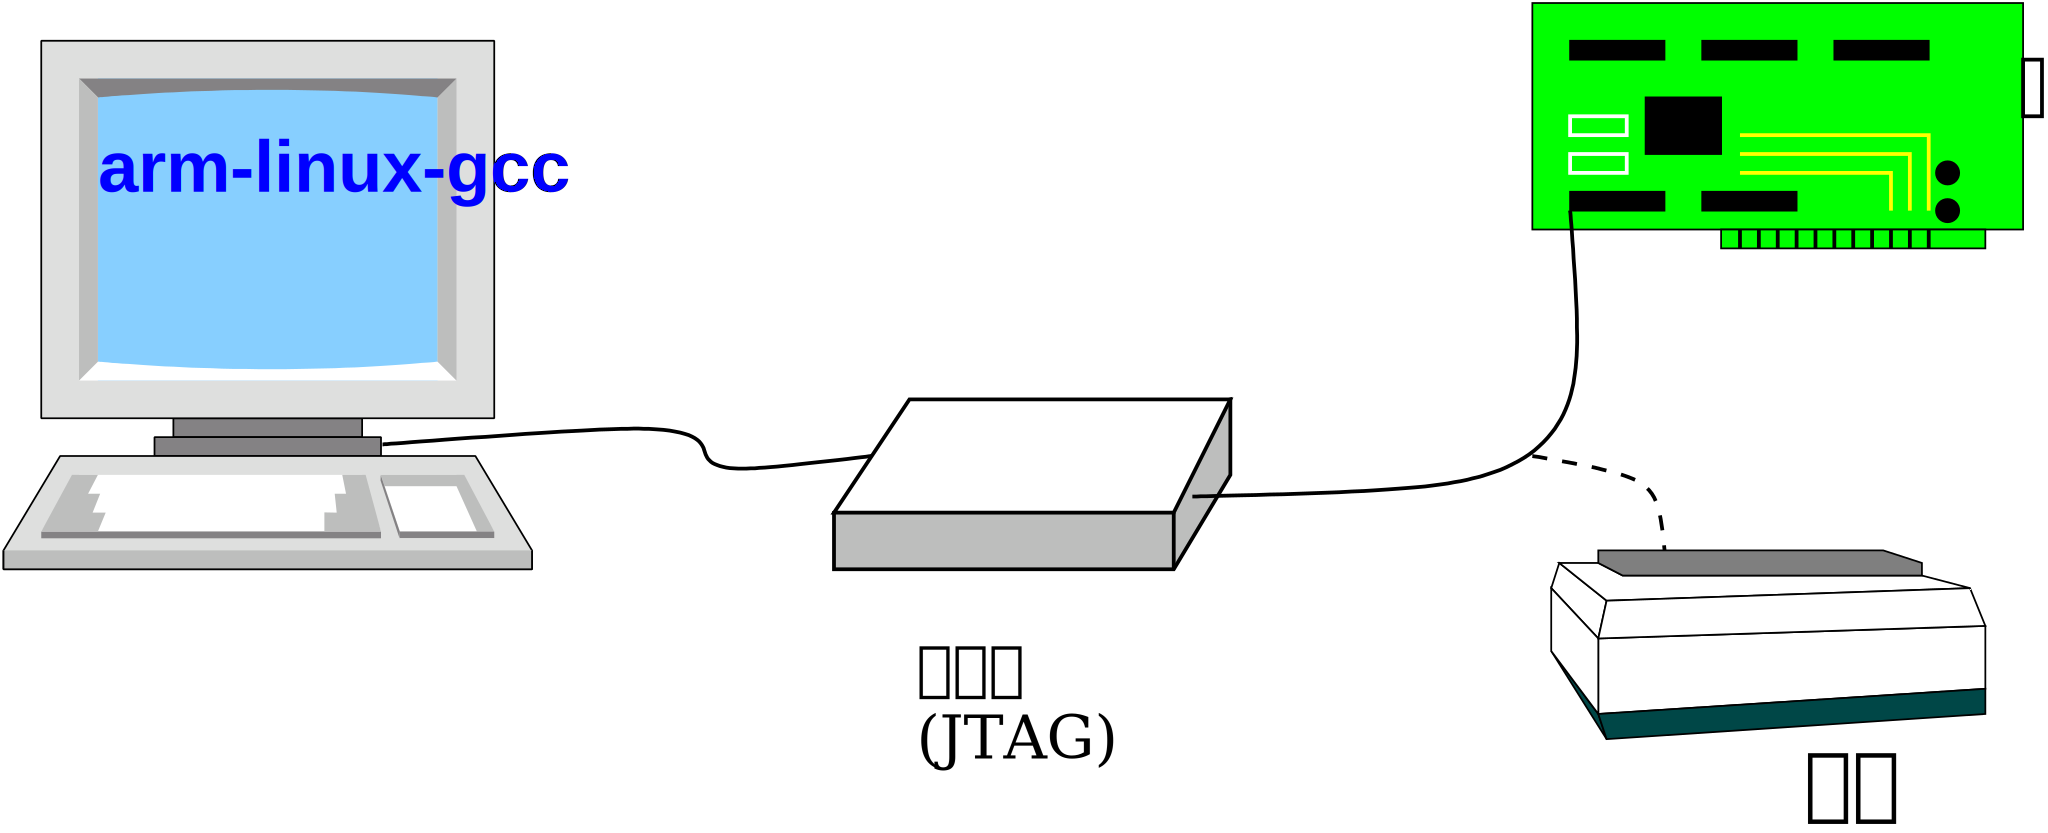
\includegraphics[width=.55\textwidth]{host-obj}
\caption{宿主机/目标机的开发模式}
\end{figure}

利用宿主机编辑工具、交叉编译器开发软件,\\
通过下载工具或其它联接方式传到目标机使之运行。
\endslide

\slide{启动minicom}
实验板上电后自动启动bootloader(bootloader可通过其他工具烧写),
并支持RS232和tftp两个协议
\begin{itemize}
  \item 主机运行minicom,该程序通过串口(RS232)和目标机连接。
  \item \textcolor{red}{minicom -s}表示对串口进行设置,普通用户不需要做这一步
  \item 串口设置 /dev/ttyS0、bps=115200、8位数据、无校验、无流控制
  \item bootloader启动后会向终端送出显示信息
  \item bootloader提示符下面可设定本机IP、宿主机IP、引导方式、启动参数等
\end{itemize}
\endslide

\slide{Boot的必要设置}
\begin{itemize}
  \item 配置IP\\
        配置目标机的IP、tftp服务器的IP(你能够控制的主机)

      x210 \# set ipaddr xxx.xxx.xxx.xxx (target IP)

      x210 \# set serverip xxx.xxx.xxx.xxx (tftp server IP)
  \item 主机和目标机互相 \textcolor{red}{ping}
  \item 配置启动选项(内核地址、文件系统、监控终端等等)

      x210 \# set bootargs ...
\end{itemize}
\endslide

\slide{tftp服务}
\begin{itemize}
  \item tftp使用UDP协议
  \item tftp的目的是为了通过网络加载Linux操作系统内核及根文件系统
  \item tftp的设置脚本文件在 /etc/xinet.d/tftp, 它设置了 tftp 的服务器目录
  \item 重启tftp服务(包括其它由xinet管理的服务)可以执行\\
        \# /etc/rc.d/init.d/xinetd restart
\end{itemize}
\endslide

\slide{加载Linux内核}
基本 Linux 操作系统由两个文件构成
\begin{itemize}
  \item \textcolor{red}{zImage} --- kernel

      x210 \# tftp 0x30008000 zImage
  \item \textcolor{red}{ramdisk\_img...}  --- file system(ext2fs)

      x210 \# tftp 0x40000000 ramdisk\_img.gz
\end{itemize}
加载成功后可通过bootloader的命令烧入FLASH,也可通过内存方式直接引导启动。

   x210 \# bootm 0x30008000
\endslide

\slide{熟悉Linux环境}
\begin{itemize}
  \item 配置目标机的IP: ifconfig
  \item 主机和目标机之间互相 \textcolor{red}{ping}
  \item 尝试用另外的窗口或终端从主机 telnet 到目标机
  \item 熟悉目标机的 Linux 环境
  \item 尝试运行其它 Linux 命令
\end{itemize}
\endslide

\slide{架设NFS服务}
\begin{itemize}
  \item NFS服务的目的是将主机上的一个目录用来和目标机共享,作为目标机的存储设备
  \item NFS服务器的目录及权限设置在文件 /etc/exports 中
  \item 主机作为NFS服务器,需要启动 nfsserver 和 portmap 两个服务
  \item 目标机上执行 mount 命令 将指定 IP 下的 NFS 共享目录挂载到 /mnt 目录
  \item 在主机和目标机上分别观察、操作共享目录下的文件
\end{itemize}
\endslide

\slide{编写应用程序}
\begin{itemize}
  \item 在主机上编写一个简单的c程序并编译、运行
  \item 将可执行程序复制到 NFS 共享目录下,尝试在目标机上运行该程序
  \item \textcolor{red}{???}
  \item 在主机上用 arm-linux-gcc 编译器编译, 再尝试用两边的机器分别运行
  \item \textcolor{red}{!!!}
  \item 在目标机上编译......$\! @\#\$\%\&*()$
\end{itemize}
\textcolor{red}{养成写``Makefile''的好习惯(事半功倍)}
\endslide

\slide{源码获取}
\begin{itemize}
  \item 本机提供内核和 busybox 源码, 在 /usr/src/x210v3 目录下
  \item 内核源码用于编译生成内核镜像文件 zImage
  \item busybox 编译后用于构成根文件系统的一部分
  \item 其他移植软件可从互联网下载
  \item 建议在 /home/student 目录下建立自己的主目录
\end{itemize}
\endslide

\slide{Trouble Shooting---串口控制}
\begin{itemize}
  \item minicom 打不开\\
		检查是否本机已经运行了一个 minicom。串行口硬件设备不允许资源共享。
  \item minicom 无法访问实验板, 或出现乱码
  \begin{itemize}
	\item 检查硬件连接(电源、串口线、串口位置)
	\item 是否以普通用户方式尝试更改 minicom 的配置(--s选项)
	\item 串口协议参数是否正确
	\item 删除主目录下的 .minirc.dfl、minicom.log 再试
  \end{itemize}
\end{itemize}
\endslide

\slide{Trouble Shooting---下载}
\begin{itemize}
  \item 无法下载内核
  \begin{itemize}
	\item 网络设置是否正确?主机与目标机能否互相 ping 通
	\item bootloader默认的文件名是否正确?
	\item 要下载的文件是否存在, 是否有读取的权限?
	\item 是否开启了主机防火墙
\end{itemize}
\end{itemize}
\endslide

\slide{Trouble Shooting---启动}
\begin{itemize}
  \item 启动与预期现象不符\\
		是否设错了启动选项,使用了不同的根文件系统?\\
		bootloader 中是否设错了 tftp 服务器地址, 用了别人的内核?
  \item 启动后无法获得终端\\
		文件系统中缺少必要的设备
  \item 无法挂载 NFS 服务器的共享目录
  \begin{itemize}
	\item 网络设置是否正确?主机与目标机能否互相 ping 通
	\item 主机 NFS 服务是否开放
	\item 目标机文件系统是否有写权限
  \end{itemize}
\end{itemize}
\endslide

\chapter{实验要求}{}
\begin{itemize}
  \item 实验环境+操作系统移植 ({\red 必做})
  \item 图形用户接口 ({\red 必做})
  \item 设备驱动(按键、LED、Buzz等) ({\red 必做})
  \item 音频接口及数据采集处理
  \item 嵌入式系统应用软件移植
  \item 扩展实验、综合实验
\end{itemize}
除必做实验以外,必须再完成至少一个选做实验。
\endslide

\slide{实验要求}
\begin{enumerate}
  \item 预习,制定实验方案,充分利用实验室时间
  \item 实验操作规范
  \item 实验记录完整详尽
  \item 善于发现问题
\end{enumerate}
\endslide

\slide{实验报告要求}
\begin{enumerate}
  \item 原理性的内容简述
  \item 实验过程详细,有根据,与原理结合,避免流水帐式的记录
  \item 对实验结果的分析讨论
  \item 附上经实验指导教师签字的原始实验记录
  \item 参考文献(参考来源)
  \item {\bf 避免成段地抄袭书本内容(无论是文字叙述还是程序代码)}
  \item 格式规范,篇幅适当(12页以内)
\end{enumerate}
\endslide
